
\chapter{Discussion}
\label{cha:discussion}

\section{Observation}
Difference between levels that are easy for humans and computers.

\subsection{Patterns}
Some levels contains an overall pattern which humans will easily spot while the computer will have a hard time solving the puzzle. A pattern could be where the player has to push the boxes in chain reaction.

An example of this is shown in \ref{fig:level7}. A human player will quite fast spot that the level is build up by a circle of boxes only moveable by moving one of the bottom boxes to the midle and then by moving the box above its startposition one square down. Following this direction around the circle all the boxes can be put onto a goal square. The computer will have to try alot of moves before finding the correct pattern.

\begin{figure}[htp]
	\centering
	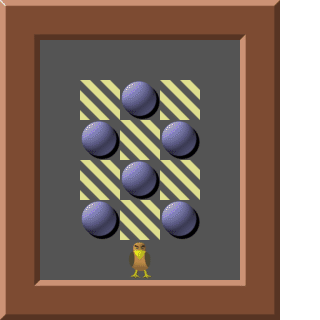
\includegraphics[scale=0.5]{level7}
	\caption{Level 7 - a level with a pattern easy to spot for a human}
	\label{fig:level7}
\end{figure}

\subsection{Deadlock detection}
Solving Sokobano puzzles is much about avoiding deadlocked states. As
it can be hard to describe when a state contains a deadlock and hard
to check if it has one in a very short time, human players might be
better at spotting these states. Though the computer would ``just''
need a better deadlock detection than what we have been able to come
up with.

\section{Improvements}
\section{More deadlock detection}
To improve the algorithm, better deadlock detections must be
created. The first to implement would be heuristics that detect the
states in figure \ref{fig:missingdeadlocks}.

First of all it should not be allowed to put two boxes into the same
narrow corridor as you cannot get in between the boxes thus making the
boxes deadlock. (The left image in figure \ref{fig:missingdeadlocks}.)
One way of solving this could be to make the corridor a one box only
zone and lock it as soon as a box is inside it.

Furthermore a deadlock detector that is able to check if a room with
only one entrance is getting blocked, must be created. (The right
image). There are many aspects in this: first of all how do you find
areas with only one entrance? And how do you decide whther the
entrance is blocked? And how do you do this without making the
algorithm very slow?

\begin{figure}[htp]
  \centering
  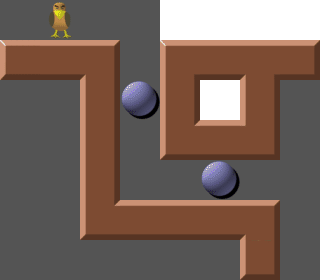
\includegraphics[width=0.4\textwidth]{blockednarrow}
  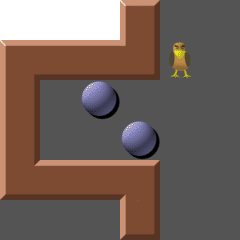
\includegraphics[width=0.4\textwidth]{blockedentrance}
  \caption{Deadlocks not found by our heuristics}
  \label{fig:missingdeadlocks}
\end{figure}


POP planning, regression planning?

Variants of sokoban
\begin{itemize}
\item Colored boxes
\item Several Pushers
\item Push rows of boxes
\item Traps/doors
\end{itemize}
